\section{Задание 6. Работа с командой строкой ОС Ubuntu.}

команда прехода по папкам \ref{fig:comandCD}, вывод текста\ref{fig:comandECHO}, удаление файла \ref{fig:comandRM}, перенос файла на одну папку назад \ref{fig:comandMV}

\begin{figure}[!h]
    \centering
    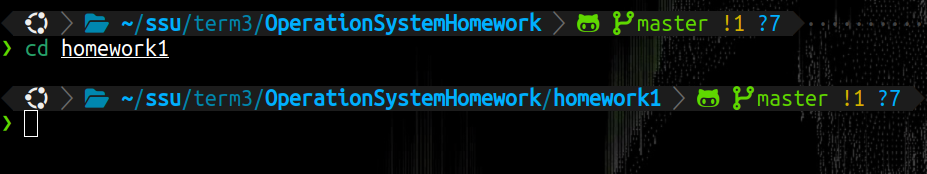
\includegraphics[width = 0.8\textwidth]{images/comandCD.png}
    
    \caption{переход по папкам}
    
    \label{fig:comandCD}
\end{figure}

\begin{figure}[!h]
    \centering
    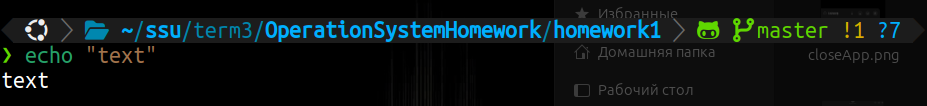
\includegraphics[width = 0.8\textwidth]{images/comandECHO.png}
    
    \caption{вывод текста}
    
    \label{fig:comandECHO}
\end{figure}

\begin{figure}[!h]
    \centering
    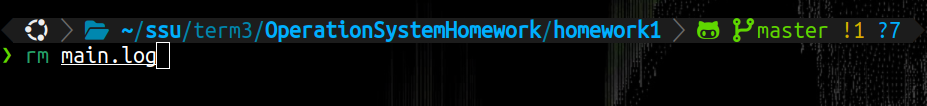
\includegraphics[width = 0.8\textwidth]{images/comandRM.png}
    
    \caption{удаление файла}
    
    \label{fig:comandRM}
\end{figure}

\begin{figure}[!h]
    \centering
    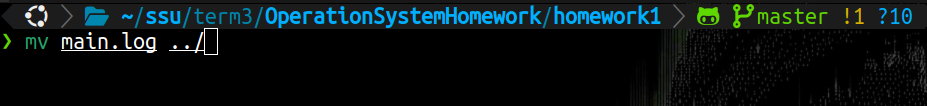
\includegraphics[width = 0.8\textwidth]{images/comandMV.png}
    
    \caption{перенос файла на одну папку назад}
    
    \label{fig:comandMV}
\end{figure}
